% 2002 年上海理科第 17 题：直三棱柱空间图
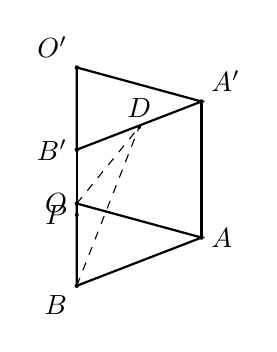
\begin{tikzpicture}[>=stealth, scale=0.72]
  \coordinate (O) at (0,0);
  \coordinate (A) at (2.2,-0.6);
  \coordinate (B) at (0,-1.45);
  \coordinate (Op) at (0,2.4);
  \coordinate (Ap) at (2.2,1.8);
  \coordinate (Bp) at (0,0.95);
  \coordinate (D) at (1.1,1.35);
  \coordinate (P) at (0,-0.2);
  \draw[thick] (O)--(A)--(B)--cycle;
  \draw[thick] (Op)--(Ap)--(Bp)--cycle;
  \draw[thick] (O)--(Op) (A)--(Ap) (B)--(Bp);
  \draw[dashed] (O)--(D) (B)--(D);
  \draw[thick] (O)--(P);
  \fill (O) circle (1.1pt) node[left] {$O$};
  \fill (A) circle (1.1pt) node[right] {$A$};
  \fill (B) circle (1.1pt) node[below left] {$B$};
  \fill (Op) circle (1.1pt) node[above left] {$O'$};
  \fill (Ap) circle (1.1pt) node[above right] {$A'$};
  \fill (Bp) circle (1.1pt) node[left] {$B'$};
  \fill (D) circle (1.0pt) node[above] {$D$};
  \fill (P) circle (1.0pt) node[left] {$P$};
\end{tikzpicture}
